% Author: Izaak Neutelings (July 2018)
% page 8 https://archive.org/details/StaticAndDynamicElectricity
% https://tex.stackexchange.com/questions/56353/extract-x-y-coordinate-of-an-arbitrary-point-on-curve-in-tikz
% https://tex.stackexchange.com/questions/412899/tikz-calculate-and-store-the-euclidian-distance-between-two-coordinates

\documentclass[border=3pt,tikz]{standalone}
\usepackage{physics,bm}
\usepackage{tikz,pgfplots}
\tikzset{>=latex} % for LaTeX arrow head
\pgfplotsset{compat=1.13}
\usetikzlibrary{decorations.markings,intersections,calc}
\usepackage[outline]{contour} % glow around text
\usetikzlibrary{angles,quotes} % for pic (angle labels)
\usepackage{xcolor}
\colorlet{Ecol}{orange!90!black}
\colorlet{EcolFL}{orange!80!black}
\colorlet{Bcol}{blue!90!black}
\tikzstyle{EcolEP}=[blue!80!white]
\colorlet{veccol}{green!45!black}
\tikzstyle{charge+}=[very thin,top color=red!50,bottom color=red!90!black,shading angle=20]
\tikzstyle{charge-}=[very thin,top color=blue!50,bottom color=blue!80,shading angle=20]
\tikzstyle{vector}=[->,thick,veccol]
\tikzset{EFieldLineArrow/.style={EcolFL,decoration={markings,mark=at position #1 with {\arrow{latex}}},
                                 postaction={decorate}},
         EFieldLineArrow/.default=0.5}
\def\R{1.8}
\def\NE{8}
\def\NV{4}
\contourlength{1.6pt}



\begin{document}


% POINT CHARGE +1
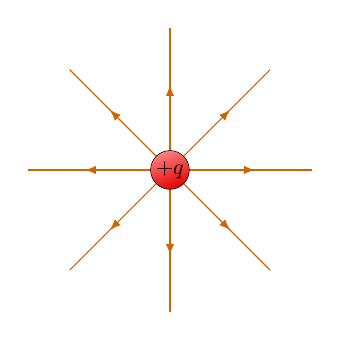
\begin{tikzpicture}
  \foreach \i [evaluate={\angle=(\i-1)*360/\NE;}] in {1,...,\NE}{
    \draw[EFieldLineArrow={0.6}] (0,0) -- (\angle:\R);
  }
  \draw[charge+] (0,0) circle (7pt) node[black,scale=0.8] {$+q$};
\end{tikzpicture}


% POINT CHARGE -1
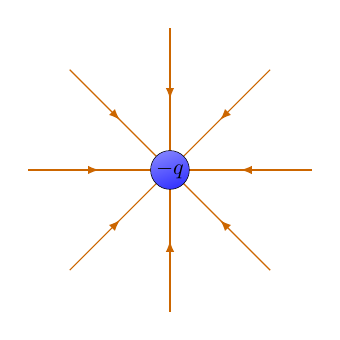
\begin{tikzpicture}
  \foreach \i [evaluate={\angle=(\i-1)*360/\NE;}] in {1,...,\NE}{
    \draw[EFieldLineArrow={0.5}] (\angle:\R) -- (0:0);
  }
  \draw[charge-] (0,0) circle (7pt) node[black,scale=0.8] {$-q$};
\end{tikzpicture}


% POINT CHARGE +1 - equipotential
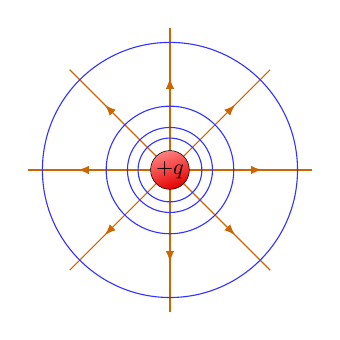
\begin{tikzpicture}
  \foreach \i [evaluate={\angle=(\i-1)*360/\NE;}] in {1,...,\NE}{
    \draw[EFieldLineArrow={0.65}] (0,0) -- (\angle:\R);
  }
  \foreach \i [evaluate={\r=0.9*\R/\i;}] in {1,...,\NV}{
    \draw[EcolEP] (0,0) circle (\r);
  }
  \draw[charge+] (0,0) circle (7pt) node[black,scale=0.8] {$+q$};
\end{tikzpicture}


% POINT CHARGE -1 - equipotential
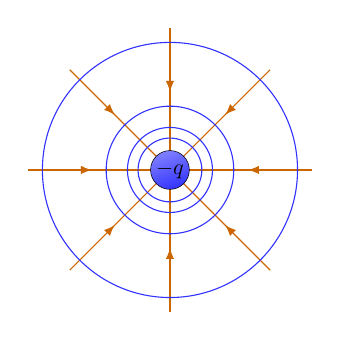
\begin{tikzpicture}
  \foreach \i [evaluate={\angle=(\i-1)*360/\NE;}] in {1,...,\NE}{
    \draw[EFieldLineArrow={0.45}] (\angle:\R) -- (0,0);
  }
  \foreach \i [evaluate={\r=0.9*\R/\i;}] in {1,...,\NV}{
    \draw[EcolEP] (0,0) circle (\r);
  }
  \draw[charge-] (0,0) circle (7pt) node[black,scale=0.8] {$-q$};
\end{tikzpicture}


% POINT CHARGE +1 - integration
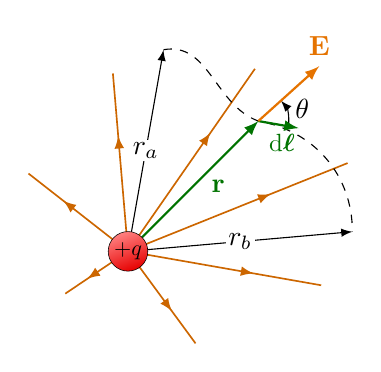
\begin{tikzpicture}[scale=1.3]
  \def\NE{7}
  \def\R{2.0}
  \def\a{1.6}
  \def\b{1.4}
  \coordinate (O) at (0,0);
  \coordinate (P) at (45:0.9*\R);
  \coordinate (L) at ($(P)+(-10:0.20*\R)$);
  \coordinate (E) at ($(P)+(42:0.4*\R)$);
  \foreach \i [evaluate={\ang=15+(\i-1)*360/\NE;}] in {1,...,\NE}{
    \draw[EFieldLineArrow={0.65},line width=0.6] (0,0) -- ({0.3*\R+\a*cos(\ang)},{0.25*\R+\b*sin(\ang)});
  }
  \draw[->] (O) -- (80:1.0*\R) coordinate (A) node[midway,fill=white,inner sep=1] {$r_a$};
  \draw[->] (O) -- (5:1.1*\R) coordinate (B) node[midway,fill=white,inner sep=1] {$r_b$};
  \draw[thin,dashed] (A) to[out=10,in=160] (P) to[out=-10,in=90] (B);
  \draw[vector] (O) -- (P) node[midway,right=9,below=-6] {$\vb{r}$};
  \draw pic[->,"$\theta$",draw=black,angle radius=11,angle eccentricity=1.5] {angle = L--P--E};
  \draw[vector] (P) -- (L) node[above=2,left=6,below=1,scale=0.9] {$\dd{\bm{\ell}}$};
  \draw[vector,Ecol] (P) -- (E) node[above] {$\vb{E}$};
  \draw[charge+] (O) circle (5.5pt) node[black,scale=0.8] {$+q$};
\end{tikzpicture}


% POINT CHARGE +1 - potential
\def\NE{7}
\def\a{0.04*\R}
\def\R{1.8}
\begin{tikzpicture}[scale=1.3]
  \foreach \i [evaluate={\angle=15+(\i-1)*360/\NE;}] in {1,...,\NE}{
    \draw[EFieldLineArrow={0.65},line width=0.6] (0,0) -- (\angle:\R);
  }
  \draw[charge+] (0,0) circle (5.5pt) node[black,scale=0.8] {$+q$};
  \draw[thin] (90:0.88*\R) coordinate (A) --++ (\a,0) --++ (-2*\a,0) node[above=2,left=-1] {$a$};
  \draw[thin] (90:0.36*\R) coordinate (B) --++ (\a,0) --++ (-2*\a,0) node[above=4,left=-1] {$b$};
  \draw[->] (A) -- (B) node[midway,above=-5] {\contour{white}{$h$}};
\end{tikzpicture}


% POINT CHARGE -1 - potential
\begin{tikzpicture}[scale=1.3]
  \foreach \i [evaluate={\angle=15+(\i-1)*360/\NE;}] in {1,...,\NE}{
    \draw[EFieldLineArrow={0.65},line width=0.6] (0,0) -- (\angle:\R);
  }
  \draw[charge-] (0,0) circle (5.5pt) node[black,scale=0.8] {$-q$};
  \draw[thin] (90:0.88*\R) coordinate (A) --++ (\a,0) --++ (-2*\a,0) node[above=2,left=-1] {$a$};
  \draw[thin] (90:0.36*\R) coordinate (B) --++ (\a,0) --++ (-2*\a,0) node[above=4,left=-1] {$b$};
  \draw[->] (A) -- (B) node[midway,above=-5] {\contour{white}{$h$}};
\end{tikzpicture}


\end{document}
